% ME3050 -  Dynamics Modeling and Controls - Tennessee Technological University
% Tristan Hill - Spring 2020 - Summer 2020 - Spring 2022
% Dynamics Modeling and Controls
% Lecture Module - Electrical Systems - Topic 4  - Mechatronics Applications

% Document settings

\documentclass{beamer}                  % for presentation ?
%\documentclass[handout]{beamer}  % for handout ?
 
%\usepackage{/home/thill/Documents/lectures/dmc_lectures/dmc_lectures}
\usepackage{/home/tntech.edu/thill/courses/dmc/dmc_lectures}

\newcommand{\MNUM}{2\hspace{2mm}} % Module number
\newcommand{\TNUM}{4\hspace{2mm}} % Topic number 
\newcommand{\moduletitle}{Electrical Systems} % Titles and Stuff
\newcommand{\topictitle}{Mechatronics Applications} 

\newcommand{\sectiontitleI}{What is Mechatronics?} % More Titles and Stuff
\newcommand{\sectiontitleII}{Example: DC Motor}
\newcommand{\sectiontitleIII}{Governing Equations}
\newcommand{\sectiontitleIV}{Model Derivation}
\newcommand{\sectiontitleV}{Response Equation}

\author{ME3050 - Dynamic Modeling and Controls}
\title{Lecture Module - \moduletitle}
\date{Mechanical Engineering\vspc Tennessee Technological University}

\begin{document}
	
	\lstset{language=MATLAB,basicstyle=\ttfamily\small,showstringspaces=false}
	
	\frame{\titlepage \center\begin{framed}\Large \textbf{Topic \TNUM - \topictitle}\end{framed} \vspace{5mm}}
	
	% Section 0 - Outline
\frame{
	
	\large \textbf{\moduletitle} \vspace{3mm}\\
	
	\begin{itemize}
	
		\item \hyperlink{sectionI}{\sectiontitleI} \vspc % Section I
		\item \hyperlink{sectionII}{\sectiontitleII} \vspc % Section II
		\item \hyperlink{sectionIII}{\sectiontitleIII} \vspc %Section III
		\item \hyperlink{sectionIV}{\sectiontitleIV} \vspc %Section IV	
		\item \hyperlink{sectionV}{\sectiontitleV} \vspc %Section V
	
	\end{itemize}

}

% Section I
\section{\sectiontitleI}

	% Section I - Frame I
	\begin{frame}[label=sectionI] \small
		\frametitle{\sectiontitleI}

		
		\btVFill
		\tiny{System Dynamics, Palm, 4$^{th}$}	

	\end{frame}

	%\section{\sectiontitleII}	
	
	% Section I - Frame II
	\begin{frame}[label=sectionI] \small
		\frametitle{\sectiontitleI}
		%\bigskip
		

		\btVFill
		\tiny{System Dynamics, Palm, 4$^{th}$}		
		
	\end{frame}

% Section II
\section{\sectiontitleII}
	
	% Section II - Frame I
	\begin{frame}[label=sectionII,containsverbatim] \small
        \frametitle{\sectiontitleII}
		Armature Controlled Brushed DC Motor \vspc

		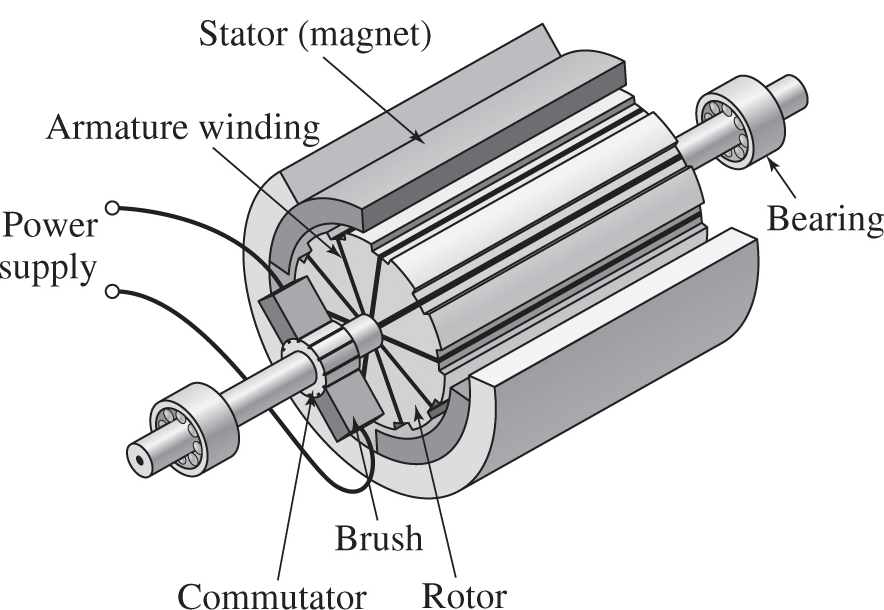
\includegraphics[scale=.85]{paL40056_06_05_03_cropped.png}

		\btVFill
		\tiny{Image: System Dynamics, Palm, 4$^{th}$, Pg. 376-378}
		
	\end{frame}

	% Section II - Frame I
	\begin{frame}[label=sectionII,containsverbatim] \small
        \frametitle{\sectiontitleII}
		Armature Controlled Brushed DC Motor \vspc

		\begin{multicols}{2}

		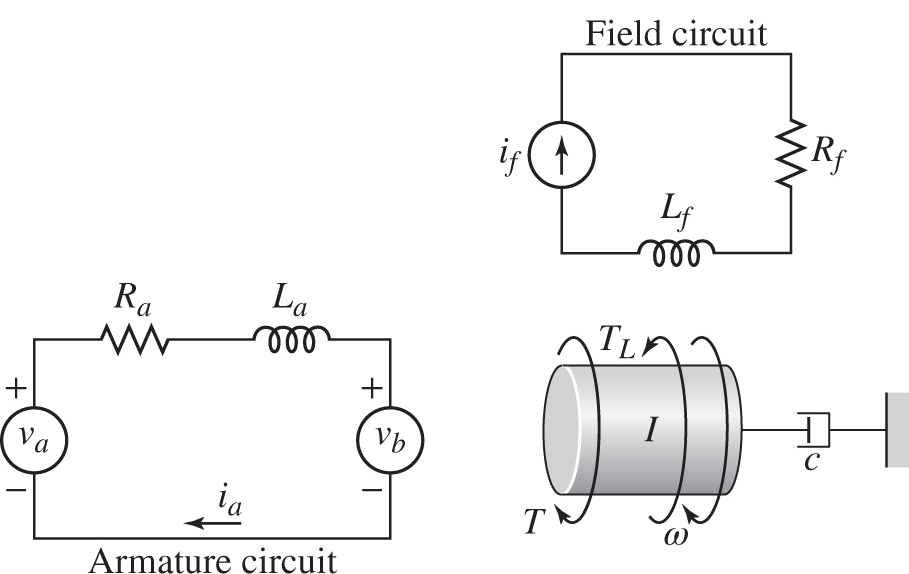
\includegraphics[scale=.65]{paL40056_06_05_04_cropped.png}
		$v_a$ : armature voltage (input)\vspc
        $R_a$ : armature resistance

        Torque on armature
        \[T=\left(nBLi_a \right)r=\left(nBLr\right)i_a=K_Ti_a \hspc (6.5.3) \] 
        Back EMF (electromotive force) voltage
        \[v_b=nBLv=\left(nBLr\right)\omega=K_b\omega \hspc (6.5.4)\]	

        \end{multicols}

		\btVFill
		\tiny{Image: System Dynamics, Palm, 4$^{th}$, Pg. 376-378}
		
	\end{frame}

	% Section II - Frame II
	\begin{frame}[label=sectionII,containsverbatim] \small
        \frametitle{\sectiontitleII}
		Armature Controlled Brushed DC Motor \vspc

		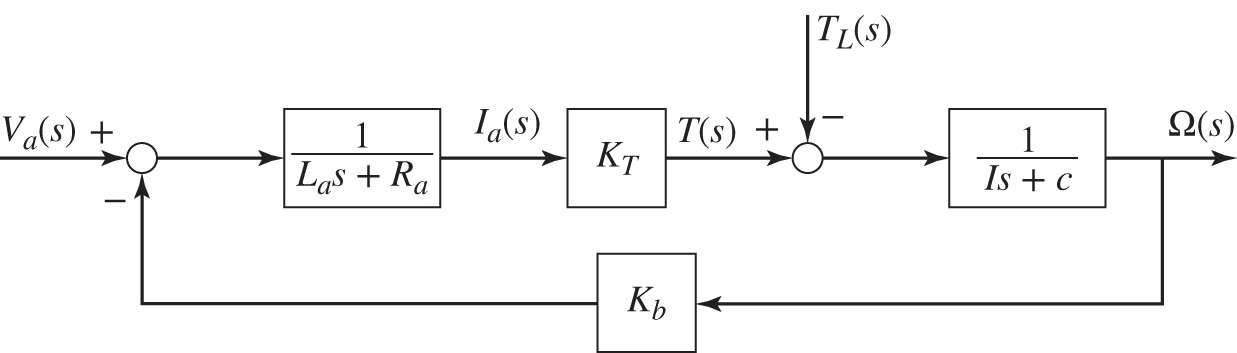
\includegraphics[scale=.65]{paL40056_06_05_05_cropped.png}

        Kirchoff's Voltage Law 
        \[ v_a-R_ai_a-L_a\frac{di_a}{dt}-K_b\omega=0 \hspc (6.5.5)\] 

        Newtons's Second Law  
        \[ I\frac{d\omega}{dt}=T-c\omega-T_L=K_Ti_a-c\omega-T_L\hspc (6.5.4)\]	

		\btVFill
		\tiny{Image: System Dynamics, Palm, 4$^{th}$, Pg. 376-378}
		
	\end{frame}	

	%Section II - Frame III
	\begin{frame} \small
		\frametitle{\sectiontitleII}

		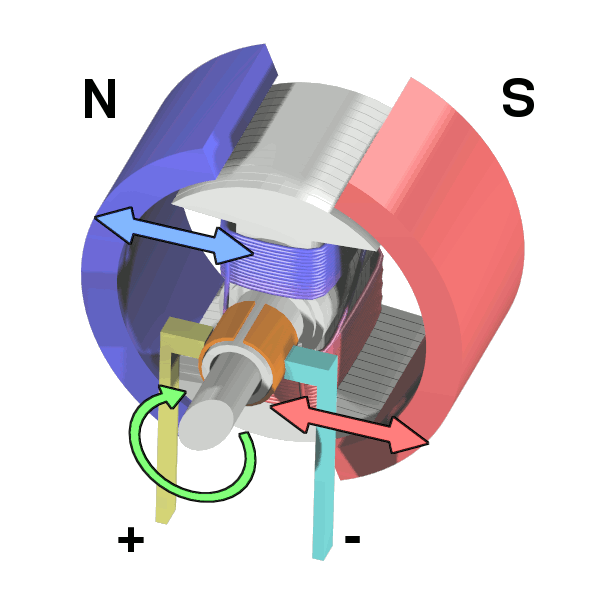
\includegraphics[scale=.25]{Electric_motor_cycle_2.png}

		\href{https://en.wikipedia.org/wiki/DC_motor}{Animation on Web} 

		\btVFill
		\tiny{source: \href{https://en.wikipedia.org/wiki/DC_motor}{wikipedia}}
	\end{frame}	

% Section III
\section{\sectiontitleIII}

	% Section III - Frame I
	\begin{frame}[label=sectionIII] \small
		\frametitle{\sectiontitleIII}
		

		\btVFill
	\end{frame}	
	
	%Section III - Frame II
	\begin{frame} \small
		\frametitle{\sectiontitleIII}
		
		\btVFill
	\end{frame}	

	%Section III - Frame III
	\begin{frame} \small
		\frametitle{\sectiontitleIII}

		

			
	\end{frame}	

% Section IV
\section{\sectiontitleIV}

	% Section IV - Frame I
	\begin{frame}[label=sectionIV] \small
		\frametitle{\sectiontitleIV}
		
	\end{frame}	

% Section V
\section{\sectiontitleV}

	% Section V - Frame I
	\begin{frame}[label=sectionV] \small
		\frametitle{\sectiontitleV}
		
	\end{frame}	

\end{document}



